\documentclass[letterpaper,12pt]{article}
\usepackage{array}
\usepackage{threeparttable}
\usepackage{geometry}
\geometry{letterpaper,tmargin=1in,bmargin=1in,lmargin=1.25in,rmargin=1.25in}
\usepackage{fancyhdr,lastpage}
\pagestyle{fancy}
\lhead{}
\chead{}
\rhead{}
\lfoot{}
\cfoot{}
\rfoot{\footnotesize\textsl{Page \thepage\ of \pageref{LastPage}}}
\renewcommand\headrulewidth{0pt}
\renewcommand\footrulewidth{0pt}
\usepackage[format=hang,font=normalsize,labelfont=bf]{caption}
\usepackage{listings}
\lstset{frame=single,
  language=Python,
  showstringspaces=false,
  columns=flexible,
  basicstyle={\small\ttfamily},
  numbers=none,
  breaklines=true,
  breakatwhitespace=true
  tabsize=3
}
\usepackage{amsmath}
\usepackage{amssymb}
\usepackage{amsthm}
\usepackage{harvard}
\usepackage{setspace}
\usepackage{float,color}
\usepackage[pdftex]{graphicx}
\usepackage{hyperref}
\hypersetup{colorlinks,linkcolor=red,urlcolor=blue}
\theoremstyle{definition}
\newtheorem{theorem}{Theorem}
\newtheorem{acknowledgement}[theorem]{Acknowledgement}
\newtheorem{algorithm}[theorem]{Algorithm}
\newtheorem{axiom}[theorem]{Axiom}
\newtheorem{case}[theorem]{Case}
\newtheorem{claim}[theorem]{Claim}
\newtheorem{conclusion}[theorem]{Conclusion}
\newtheorem{condition}[theorem]{Condition}
\newtheorem{conjecture}[theorem]{Conjecture}
\newtheorem{corollary}[theorem]{Corollary}
\newtheorem{criterion}[theorem]{Criterion}
\newtheorem{definition}[theorem]{Definition}
\newtheorem{derivation}{Derivation} % Number derivations on their own
\newtheorem{example}[theorem]{Example}
\newtheorem{exercise}[theorem]{Exercise}
\newtheorem{lemma}[theorem]{Lemma}
\newtheorem{notation}[theorem]{Notation}
\newtheorem{problem}[theorem]{Problem}
\newtheorem{proposition}{Proposition} % Number propositions on their own
\newtheorem{remark}[theorem]{Remark}
\newtheorem{solution}[theorem]{Solution}
\newtheorem{summary}[theorem]{Summary}
%\numberwithin{equation}{section}
\bibliographystyle{aer}
\newcommand\ve{\varepsilon}
\newcommand\boldline{\arrayrulewidth{1pt}\hline}


\begin{document}

\begin{flushleft}
  \textbf{\large{Problem Set \#1}} \\
  OSM Lab, Dr. Evans \\
  Dan Ehrlich
\end{flushleft}

\vspace{5mm}

\noindent\textbf{Problem 1}
Solving for the steady state we find that the steady state values are:
$$\bar{b_2} = 0.01931274$$ 
$$\bar{b_3} = 0.05841159$$ 
$$\bar{c_1} =0.18241256	$$
$$\bar{c_2} =0.20961491	$$
$$\bar{c_3} =	0.24087382$$
$$\bar{w} = 0.20172529359557331	$$
$$\bar{r} = 2.4330302535646116	$$\\

\noindent\textbf{Problem 2}
Solving for the steady state when we increase $\beta$ to $0.55$ we find that the steady state values change to
$$\bar{b_2} = 0.02817696 $$ 
$$\bar{b_3} =  0.07686557$$ 
$$\bar{c_1} =0.19597535	$$
$$\bar{c_2} =0.22861559$$
$$\bar{c_3} =	0.26669216$$
$$\bar{w} =  0.22415231191003757	$$
$$\bar{r} = 1.8863599991451423 $$
We noticeably see an increase in both savings and consumption. Increase in patience means that consumers are willing to consume less now by consuming more in the future and therefore increase savings. Consumption will therefore increase as well. The interest rate, however, as expected goes down as savings go up. The wage in this case does not depend on labor decisions which are constant, and would have no doubt changed if labor was endogenous. Instead, it changes as a result of the the change in capital that results from the increase in savings.\\\\  

\noindent\textbf{Problem 3} The transition path of capital is solved for using the uploaded code and takes 129 iterations to converge. \\

\noindent\textbf{Problem 4} It takes 21 iterations to converge until the economy is within $0.0001$ of the Steady State. This accomplished by changing the $\xi$ value to $0.0001$. 

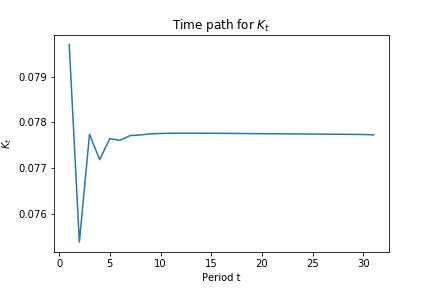
\includegraphics{TPIgraph.jpeg}

\end{document}

